% =====================================================================
%  Junior Independent Work  --  Steven Goetz, Princeton Economics
%  Skeleton: sections marked [TODO] are placeholders; the Literature
%  Review and the two Results tables are filled in.
% =====================================================================
\documentclass[12pt]{article}

\usepackage[margin=1in]{geometry}
\usepackage{setspace}
\usepackage{booktabs}          % \toprule \midrule \bottomrule in tables
\usepackage{multirow}
\usepackage{adjustbox}       % tables shrink to text width only when too wide
\usepackage{graphicx}
\usepackage{amsmath}
\usepackage{pgfplots}          % bar chart of failure rates by structural score
\pgfplotsset{compat=1.17}
\usepackage[hidelinks]{hyperref}
\usepackage{natbib}            % \citet{} and \citep{} with author-year style
\bibliographystyle{apalike}

\doublespacing

\title{Runway to Nowhere? <-> Extend and Pretend—or Mend?}
\author{Steven Goetz\\ Department of Economics, Princeton University\\
        \small Junior Independent Work, Fall 2026}
\date{\today}

\begin{document}
\maketitle

\begin{abstract}
\noindent [TODO: 150--200 words. Question, data (277 U.S. exchanges 2014--2025: 89 coercive LMEs from Roe \& Rotaru and 188 pro rata distressed exchanges from S\&P), method (a continuous 0--1 structural score built from 70 blind re-codings of each deal's pre-deal rating-agency text; failure within 1/2/3 years; LPMs with year and industry fixed effects), headline results (after a pro rata exchange, going from a pure-shock to a pure-structural firm raises two-year failure by 25 points, $p = 0.02$, smaller and less precise than under the original three-group coding; LMEs fail more often at every score; lenders' terms do not vary with the score), and what it means for lenders' consent.]
\end{abstract}

% ---------------------------------------------------------------------
\section{Introduction}
% ---------------------------------------------------------------------
% Source: ECO 396 Literature Review, draft D2.

Corporations that cannot service their debt and run the risk of defaulting have two paths to correct their liabilities: in-court (IC) or out-of-court (OOC). While IC can eliminate more debt and offers tools like contract rejection and the automatic stay, OOC is usually the first course of action because it is quicker, cheaper, and not as frowned upon in the public eye \citep{schwartz1993, altman2019}. The newest OOC forms (uptiers, drop-downs, etc.) have been grouped under the umbrella term Liability Management Exercise (LME). The most contentious are the coercive non-pro rata LMEs, which force a minority of creditors to relinquish value so that the majority and the equity come out ahead. Sponsors and bankers praise these deals for ``extending a debtor's runway, preserving value, strengthening its balance sheet, and avoiding bankruptcy'' \citep[p.~9]{roerotaru2026}, but the newest restructuring literature points to a very different track record: roughly 40\% of these firms file within a year and over 70\% within three \citep{roerotaru2026}.

But is this fair? Is the runway an LME provides for a cruise company during the pandemic (which entered distress due to an unexpected shock in demand) just as ineffective for a floppy disk manufacturer (whose technology is obsolete)? Both may be unable to support their liabilities and employ the same OOC tactics, so is it right to pool them? Past corporate finance literature has separated distress into two buckets, financial (a sound business with too much debt) and economic (a business losing value), and runway should, in theory, help the first kind and not the second \citep{wruck1990, andrade1998}.

Thus, before completely writing off LMEs, we ask two questions. First, do post-exchange outcomes depend on the cause of the borrower's distress---a temporary shock to demand, operations, or the balance sheet versus a structural impairment of the business itself? Second, do the lenders whose consent these deals require condition their terms on that diagnosis? We expect outcomes to differ by cause and lender terms not to. Of course, these deals will keep happening regardless of efficacy because of the sponsor's incentives, but the answer is crucial for creditors, who can learn when the runway is worth signing.

The review proceeds in four parts: out-of-court restructuring and its outcomes, the incentives of the parties involved, what we have seen thus far from lenders and their contracts, and the literature that classifies the cause of distress. We then lay out the gap and our contribution.

% ---------------------------------------------------------------------
\section{Literature Review}
% ---------------------------------------------------------------------

\subsection{Out-of-court restructuring and its outcomes}

One of the main purported advantages of an OOC restructuring is that it is much less costly than Chapter 11, in both explicit (attorney fees) and indirect (demand) ways.

\paragraph{Costs of IC.} \citet{antill2026} ran three incentivized randomized experiments ($\sim$1,749 participants) to estimate the indirect costs via lost customers across airlines, car manufacturers, and retail. Learning of a Chapter 11 filing cuts a consumer's willingness to pay by 17\% to 28\% depending on the industry, implying indirect costs of 10--31\% of firm value, and these costs do not show up before the filing itself. \citet{ellias2026} covers the explicit side: Chapter 11 fees consumed roughly four times more of pre-petition assets in 2022 than in the 2010s, with the median daily cost rising from \$32k to \$84k.

\paragraph{Costs of OOC.} Distress is also expensive before anyone files. \citet{elkamhi2024} employ a dynamic trade-off model and find that pre-default costs run about 6.5\% of firm value per year and make up roughly 64\% of total distress costs.

So an LME doesn't ``automatically'' save costs. The two sides are measuring different costs at different moments: a one-time demand hit when the firm files versus a running cost for every year it stays distressed. An LME avoids the first and extends the second. It only pays off if the deal actually solves the distress, and \citet{roerotaru2026} find that it usually does not. In their hand-collected set of 89 coercive non-pro rata LMEs, aggregate debt is essentially unchanged after the deal, 88\% of firms are still rated CCC+ or below, and 71\% are in bankruptcy within three years. The firm pays the extended pre-default costs and then the Chapter 11 costs anyway.

The studies also diverge on how to measure success. \citet{roerotaru2026} use survival. \citet{harmon2026} argues the better indicator is trading prices, since a firm can survive a value-destroying deal and that should not make the strategy look successful; in his 16 LMEs, 10 destroyed value. The two methods agree, but neither can separate a value-destroying deal from a doomed firm. That distinction depends on why the firm was distressed, which neither study observes.

Nevertheless, if LMEs can double the cost (OOC and then IC) with relatively high probability, why are sophisticated players continuing them?

\subsection{Controller incentives: why the deals happen regardless}

\citet{ellias2020} blame the law. Since Delaware's \emph{Gheewalla} decision (2007), company boards owe creditors no fiduciary duties, and the equity of an insolvent firm is essentially a free call option: worthless if nothing changes, but with a positive payout in the off chance that the company rebounds. \citet{buccola2023} disagrees that the courts are at fault and puts it on private equity sponsors, who postpone filing because it would crystallize losses to their own investors and who pay little reputational cost for aggressive tactics as long as credit is cheap. The distinction matters because the remedies differ: if Ellias and Stark are right, a court ruling could change behavior; if Buccola is right, only a tighter credit market can. \citet{buccolakahan2025} sit in the middle: some coercion is efficient for overcoming holdouts, but exclusive non-pro rata uptiers are the hardest form to justify.

All three treat the proposing party's incentives as fixed, which means the sample of deals is not selected on fixability and the only decision that actually varies is the lenders' consent. So do creditors, who know sponsors will pursue paths adverse to their returns, account for this risk in their contracts?

\subsection{Do lenders and contracts respond to LME risk?}

\citet{buccolanini2024} investigate this by reading 600+ loan agreements from before and after the two landmark deals, J.Crew's drop-down (2016) and Serta's uptier (2020). Before Serta, only about 40\% of loans blocked uptiers (and often by accident); within a year after, about 75\% did. But after J.Crew, drop-down protections barely changed and only narrow ``IP blockers'' spread. Buccola and Nini suggest the flexibility to move assets is valuable to borrowers as a liquidity option, so the market may have deliberately left that door open.

\citet{badawi2024} then test whether that choice was priced: if lenders pick terms on purpose, loans vulnerable to an uptier should have traded at wider yields once uptiers proved legal and practical. Across every publicly traded loan outstanding in 2020, they find essentially no price difference between susceptible and immune loans and conclude that terms spread through lawyers and trade associations copying each other, not through prices. However, \citet{ivashina2025} find prices do move at a coarser level: across 1,240 credit agreements, carve-outs and deductibles gut covenants that look strong on paper, the weakness is concentrated in sponsor-backed and nonbank-funded loans, and weak-covenant loans fell market-wide after J.Crew. The two reconcile if lenders price contract weakness crudely and after famous shocks, not term by term.

Importantly, all of these studies look at loan origination. None looks at the later moment when a distressed borrower asks its lenders to sign an exchange, even though by then the rating agencies have published why the firm is distressed. Creditors cannot levy blockers across every company, but they could selectively decide who gets runway if they had a diagnosis to screen on.

\subsection{Classifying the cause of distress}

In fact, there are 30 years of academic research covering what ``fixable'' versus ``unfixable'' distress looks like. \citet{wruck1990} named the two kinds: financial (a good business carrying too much debt) and economic (the business itself is broken). \citet{andrade1998} measured the difference on 31 overleveraged buyouts that hit trouble: firms whose industry-adjusted operating margins held up lost almost nothing to distress, while firms whose business also declined lost 10--20\% of value. Runway for the first kind of company makes sense because the margins were never the issue; the second kind will just continue to decline unless there is a compelling reason otherwise.

Other literature in that era splits the causes further and codes them differently. \citet{asquith1994} decompose the distress of 102 junk-bond issuers into an industry downturn, firm-specific underperformance, and pure leverage, and find that profitability alone does not predict who avoids Chapter 11. \citet{opler1994} add the mechanism: leverage is what turns an industry shock into firm distress. \citet{denis1995} could not get financials for their failed recapitalizations, so they coded causes from news reports and annual reports and found distress driven more by industry downturns and unexpected regulatory and macroeconomic developments than by bad firm decisions. The camps disagree on which cause dominates, likely because their samples differ, and on method because of what their samples disclosed. A modern sample has the same bind, since most exchanged issuers are private, which is why we code cause from rating-agency text and validate it with Andrade and Kaplan's margin rule on public filers.

\citet{kahl2002} is the one paper that predicts lenders should already be doing this. In his model, creditors cannot tell at first which kind of distress they face, so they rationally keep firms on short leashes and pull the plug as they learn. Extend-and-PIK deals look a lot like that short leash, which makes our second question a real test rather than a foregone conclusion.

\subsection{Research gap and contribution}

The literature reveals that distressed exchanges usually fail, but at the end of the day, sponsors and management will continue them because the equity trades like a call option and management keeps its control and fees until a filing \citep{roerotaru2026}, and creditors, in credit markets as tight as today's, mostly go along. The cause-of-distress literature gives an excellent classification resource, but it predates the modern forms of LMEs, and there is no evidence that creditors take it into account when signing a deal. The outcome studies pool firms, the classification studies never touched exchanges, and the lender-response studies stop at origination.

This paper fills that gap in two parts. The first applies the financial-versus-economic distinction (coded from pre-deal rating-agency rationales, validated with Andrade and Kaplan's operating-performance rule on public filers) to every S\&P-recorded U.S.\ distressed exchange from 2018 to 2025, testing whether the pooled failure rates conceal a subgroup for which runway works. The second tests whether the terms lenders require vary with that published diagnosis or only with the deal's form and vintage. If the results are null, Roe and Rotaru's conclusion extends to distressed exchanges generally. If results are present, creditors can use them as a screening tool for when to grant runway and when to insist on a haircut or control.

% ---------------------------------------------------------------------
\section{Data and Method}
% ---------------------------------------------------------------------

\subsection{Sample construction}

The analysis sample pools two sets of U.S.\ distressed exchanges completed between 2014 and 2025. Table~\ref{tab:sample} traces the construction.

\begin{table}[htbp]
\centering
\caption{Sample construction}
\label{tab:sample}
\small
\begin{tabular}{p{0.72\textwidth} r r}
\toprule
 & Excluded & Remaining \\
\midrule
\multicolumn{3}{l}{\textit{Panel A: Pro rata distressed exchanges (S\&P default studies, 2018--2025)}} \\[2pt]
Defaults by issuers in S\&P's U.S.\ region (incl.\ Bermuda and Cayman domiciles) &  & 548 \\
\quad less: defaults that were not distressed exchanges (Chapter 11, missed payment, other) & 273 & 275 \\
\quad less: operating company not U.S.-based & 10 & 265 \\
\quad less: tagged as an exchange but in fact a Chapter 11 filing (net of one reverse correction) & 2 & 263 \\
\quad less: S\&P record of a deal already in the Roe--Rotaru LME list & 54 & 209 \\
\quad less: other exchanges by Roe--Rotaru companies on non-matching dates (set aside) & 21 & 188 \\
\addlinespace
\textbf{Pro rata exchanges} (143 issuers) &  & \textbf{188} \\
\addlinespace[6pt]
\multicolumn{3}{l}{\textit{Panel B: Coercive non-pro rata LMEs (Roe \& Rotaru 2026)}} \\[2pt]
Non-pro rata LMEs by U.S.\ borrowers, 2014--2025 &  & 89 \\
\quad of which: recorded by S\&P as a distressed exchange &  & 54 \\
\quad of which: not in S\&P's tables &  & 35 \\
\qquad new-money drop-down or double-dip, not a default under S\&P's definition &  & 19 \\
\qquad closed before the 2018 study window &  & 5 \\
\qquad issuer unrated or confidentially rated &  & 6 \\
\qquad issuer outside S\&P's U.S.\ region &  & 4 \\
\qquad other &  & 1 \\
\addlinespace
\textbf{Coercive LMEs} &  & \textbf{89} \\
\midrule
\textbf{Analysis sample} &  & \textbf{277} \\
\bottomrule
\end{tabular}
\begin{minipage}{0.95\textwidth}
\vspace{4pt}\footnotesize
\textit{Notes.} Panel A starts from every default listed in S\&P Global Ratings' \textit{Annual U.S.\ Corporate Default and Rating Transition Study} for 2018 through 2025 whose issuer falls in S\&P's U.S.\ region. ``Distressed exchange'' is S\&P's own reason-for-default tag. The two mis-tagged rows are Bertucci's (April 2018) and Riverbed (November 2021); GEO Group (August 2022) was tagged Chapter 11 but was an exchange and is retained. The 21 set-aside rows are exchanges by companies that appear in the Roe--Rotaru list but on dates that do not correspond to a listed LME; they are excluded so that no issuer contributes both an LME and a pro rata exchange to the comparison. Panel B uses the Roe--Rotaru deal list as published. S\&P publishes defaults by publicly rated issuers only; confidentially rated defaulters (roughly 11--13\% of each year's total) and unrated private-credit borrowers are not observable in either panel.
\end{minipage}
\end{table}


\paragraph{Coercive LMEs.} The first set is the 89 non-pro rata liability management exercises hand-collected by \citet{roerotaru2026} from Octus, 9fin, Debtwire and CreditSights. Their definition---a transaction that requires only a lender majority and leaves non-participating creditors with a worse claim---is adopted as the sample boundary, and their deal list, dates and post-deal outcome coding are used as given.

\paragraph{Pro rata exchanges.} The second set is drawn from S\&P Global Ratings' \emph{Annual U.S.\ Corporate Default and Rating Transition Study} for 2018 through 2025, which lists every rated issuer that defaulted in the year with the date and the reason for default. S\&P treats an exchange as a default when investors receive less value than the original promise \emph{and} the exchange is undertaken to avoid a conventional default \citep[the ``distressed exchange'' criteria; see][]{roerotaru2026}, so the ``distressed exchange'' tag is S\&P's own judgment that the deal was coercive in substance rather than opportunistic. The 2018--2025 studies contain 548 defaults by issuers S\&P classifies as U.S.\ (a region that in S\&P's definition includes Bermuda and Cayman domiciles). Of these, 275 are distressed exchanges. Ten are removed because the operating company is not U.S.-based, and two because the event was in fact a Chapter 11 filing mis-tagged in the tables (Bertucci's, April 2018; Riverbed, November 2021), while one Chapter 11 tag was reversed on inspection (GEO Group, August 2022, an exchange). Of the remaining 263, 54 are the S\&P record of a deal already in the Roe--Rotaru list and 21 are \emph{other} exchanges by Roe--Rotaru companies on different dates; both are set aside so that an issuer's LME and its pro rata exchange are never counted twice. That leaves 188 pro rata distressed exchanges, which together with the 89 LMEs make up the 277-deal analysis sample.

Two features of this construction matter for interpretation. First, S\&P publishes only defaults by \emph{publicly} rated issuers; confidentially rated defaulters, roughly 11--13\% of the total in each year's study, are invisible, as are unrated private-credit borrowers. Second, 35 of the 89 Roe--Rotaru LMEs do not appear in S\&P's tables at all---19 because a new-money drop-down or double-dip is not a default under S\&P's definition, 5 because they pre-date 2018, and the rest because the issuer was unrated or non-U.S.---so the pro rata set is a comparison group of \emph{S\&P-recognised} exchanges rather than a census of all out-of-court restructurings.

\subsection{Cause-of-distress coding}

The independent variable is the cause of each firm's distress in the year before the exchange. Following \citet{wruck1990} and \citet{andrade1998}, the top-level distinction is between a firm whose business is intact but whose balance sheet is not (financial distress; group A, ``shock'') and a firm whose business itself is impaired (economic distress; group B, ``structural''), with a third group (C, ``mixed'') for firms in which an external shock landed on a pre-existing structural problem. Each group is subdivided: A1 demand or operating shock, A2 financial shock (buyout leverage, maturity wall, refinancing risk with stable EBITDA); B1 secular industry decline, B2 firm-specific deterioration, B3 legal or regulatory. The full codebook, including tie-break rules, is reproduced in Appendix~\ref{app:codebook}.

The source text is the S\&P and Moody's rating-action rationales published in the twelve months before the deal, supplemented by the agencies' statements of the EBITDA trend over the prior two years. Coding follows a directed (deductive) content-analysis protocol \citep{hsieh2005}: the categories and rules are fixed in advance, the coder identifies the \emph{primary} driver the agency names, and secondary factors do not change the letter. Three tie-break rules do most of the work. The EBITDA rule leans B when EBITDA fell by more than roughly 10\% over two years \emph{and} the agency attributes the fall to the business rather than to an external event, and leans A2 when EBITDA is flat or rising; this operationalises Andrade and Kaplan's industry-adjusted operating-performance test with the information available for private issuers. The COVID rule codes a 2020--21 deal in which the pandemic is named as primary as A1 unless the issuer had already been downgraded or placed on negative outlook for operating reasons in the 24 months before March 2020, in which case it is C. The LBO rule codes leverage from a buyout or dividend recapitalisation on a stable business as A2 rather than B2. For each deal the coder records the code, a confidence level, the primary and secondary drivers, the verbatim agency language relied on, the EBITDA trend and the sources consulted.

The first-pass codes were produced by an AI research assistant applying this codebook deal by deal, with the agency text and sources retained for every observation. Because that is a non-standard coder, Section~\ref{sec:reliability} treats it as coder~\#1 and tests it against independent re-codings.

\subsection{From codes to a structural score}
\label{sec:score}

The three-way classification has two weaknesses for estimation. The mixed group is where coder judgment enters---Section~\ref{sec:reliability} shows that independent coders reassign about half of it---and splitting an already small sample three ways leaves few deals per cell. The main specification therefore replaces the three groups with a single continuous measure. Each deal is re-coded 70 times by three language models that see only the pre-deal evidence (Section~\ref{sec:reliability}), and the \emph{structural score} is the share of those runs that code the deal structural, counting a mixed code as one half:
\begin{equation}
  \text{Score}_i = \frac{B_i + \tfrac{1}{2}\,C_i}{A_i + B_i + C_i},
  \label{eq:score}
\end{equation}
where $A_i$, $B_i$ and $C_i$ are the numbers of runs that code deal $i$ as shock, structural and mixed. A deal every coder calls shock scores 0, a deal every coder calls structural scores 1, and a deal on which the coders split, or which they call mixed, falls in between. The score treats disagreement among coders as information about the deal rather than as error to be adjudicated away, in the spirit of entering label probabilities rather than hard labels in a downstream regression \citep{egami2023}. Two of the 277 deals have no pre-deal agency text and cannot be scored, which leaves 275.

The score is bimodal. Eighty-nine deals (32\%) are coded structural by every run and 31 (11\%) shock by every run; 26\% of deals fall in the bottom third of the scale, 14\% in the middle third and 60\% in the top third. It rises across coder~\#1's groups in the expected order---among pro rata exchanges it averages 0.21 for A, 0.70 for C and 0.84 for B---but it places coder~\#1's mixed deals much closer to structural than to the midpoint. Three coarser versions are carried as robustness checks: a binary indicator for a score above one half (``majority wins''), three bins of the score, and coder~\#1's original labels.

\subsection{Coding reliability}
\label{sec:reliability}

Reliability is assessed in the way the recent literature on language models as annotators recommends \citep{gilardi2023, tornberg2024, ziems2024}: the same evidence packet is re-coded many times by several independent models, agreement is summarised with Krippendorff's $\alpha$ \citep{krippendorff2018} and Fleiss' $\kappa$ \citep{landis1977}, and the downstream estimates are re-run under each coding.

Each re-coding ``coder'' receives, for every deal, the company name, deal date and S\&P industry sector; the verbatim pre-deal agency language; the two-year EBITDA direction; the secondary factors recorded; and the codebook. It does not receive the existing code, coder~\#1's rationale, the deal's form (LME or pro rata) or anything about the outcome or the terms. Because a single run of a language model at non-zero temperature is one draw from a distribution over labels \citep{reiss2023}, each model codes each deal repeatedly and the share of runs landing on each group is used as that model's probability that the deal is A, B or C \citep[``self-consistency'';][]{wang2023}. Three models were used---gpt-4o-mini and gpt-4.1-mini with 30 runs per deal and gpt-4o with 10---for 19,310 codings of the 275 deals with agency text. The Monte-Carlo error of a share estimated from 30 runs is at most about $\pm 9$ percentage points, which is adequate for classifying deals as confidently or ambiguously coded; additional precision is better bought with additional model families, which are closer to independent coders, than with additional runs of one model.

The results are as follows. The three models agree with one another on 80--86\% of deals pairwise ($\alpha = 0.70$ among the three modal labels; $0.72$ across all individual runs), and with coder~\#1 on 65\% ($\alpha = 0.38$--$0.46$ per model, $0.56$ with all four coders). On 74\% of deals at least 80\% of the 70 runs agree. The disagreement with coder~\#1 is concentrated in the mixed group: the models reclassify 43 of coder~\#1's 82 C deals as structural, whereas on the A-versus-B distinction that Part~1 rests on agreement is 83\%. The reclassification is informative rather than noise---coder~\#1's C deals that the models move to B fail within two years at 48\%, those they leave in A or C at 14\%---which indicates that the C rule, not the shock/structural line, is where coder judgment enters. A name-leakage check in which the company is anonymised in the prompt and in the quoted text, and the date rounded to the year, changes the modal label on 9\% of deals and the probability of a structural code by 0.06 on average, so the coders are responding to the agency language and the EBITDA rule rather than to what they may already know about well-known issuers. 

For the continuous score the relevant statistics are correlations rather than $\kappa$, which is defined for categories. The three models' scores correlate 0.84--0.86 pairwise; the intraclass correlation is 0.84 for a single model and 0.94 for the three-model average that the score uses, which is ``excellent'' on the usual benchmark \citep{koo2016}; and the name-scrubbed score correlates 0.95 with the named one. The score correlates 0.57 with coder~\#1's labels placed on the same 0--1 scale. Because every coder read quotations that coder~\#1 selected, these figures are upper bounds on true inter-coder reliability. Section~\ref{sec:p1} reports the main estimate under each alternative construction of the cause measure. [TODO: hand-code a random subsample from the full rating-action text and report its agreement with the score.]

\subsection{Outcomes}

Following \citet{roerotaru2026}, a deal ``fails'' if the issuer files for Chapter 11 or completes a further distressed exchange. For the LMEs the outcome and its date are Roe and Rotaru's; for the pro rata exchanges they are taken from the issuer's later appearances in the S\&P default tables, with Chapter 11 dates verified against dockets. Outcomes are measured within $h \in \{1, 2, 3\}$ years of the deal and, to avoid comparing a 2015 deal observed for eleven years with a 2025 deal observed for months, a deal enters the $h$-year analysis only if the data cutoff (14 January 2026) lies at least $h$ years after it. Of the 277 deals, 239 are eligible at one year, 186 at two and 134 at three (237, 184 and 134 of the 275 with a structural score). Bankruptcy alone is reported alongside the combined measure. Because an issuer may appear more than once, standard errors are clustered by issuer throughout; with only eleven industry groups, clustering by industry would leave too few clusters for reliable inference \citep{cameron2015}.

\subsection{Terms of the exchange}

For Part~2, the terms of each S\&P-recorded exchange (the 188 pro rata deals and the 54 LMEs S\&P records; 242 in all) were coded from the S\&P and Moody's releases announcing the selective default and from the sources those releases cite. Sixteen fields are recorded---transaction type, treatment of non-participating holders, haircut, debt reduction, maturity extension, coupon change, new money and its priority, equity to creditors, governance rights, covenant changes, sponsor support, and the evidence and sources---and collapsed into binary flags: \texttt{haircut\_any}, \texttt{equitized}, \texttt{extension\_any}, \texttt{pik}, \texttt{coupon\_up}, \texttt{new\_money\_any}, \texttt{nm\_priming} (new money that primes existing lenders), \texttt{equity\_control}, \texttt{governance}, \texttt{docs\_tight}, \texttt{docs\_loose}, \texttt{sponsor\_support} and \texttt{non\_pro\_rata\_terms}. A flag is missing, not zero, when the release does not address that term, and every share reported is computed over deals where the term is stated. Forty open-market repurchases, which carry no lender-imposed terms, are excluded, leaving 200 negotiated deals (148 pro rata, 52 LMEs).

Two kinds of summary measure are used. The first are simple counts: a control index (0--5: haircut, control equity, governance rights, documents tightened, priming lender new money), an ownership index (0--3) and a runway index (0--4: extension, PIK, documents loosened, sponsor support), together with a relief-type classification into \emph{balance-sheet fix} (haircut or equitisation) and \emph{runway only} (extension or PIK with no haircut). Because a count treats an unstated term as absent and rewards deals whose releases happen to mention more terms, the second is a standardised strictness index: each flag is $z$-scored over the deals where it is stated, signed so that higher always means tougher on the borrower (the four runway terms enter negatively), and averaged over whatever components are observed for the deal \citep{kling2007}; an inverse-covariance-weighted version \citep{anderson2008} is reported as well. The strictness index is defined for all 148 negotiated pro rata deals.

\subsection{Specifications}

The main Part~1 specification is a linear probability model,
\begin{equation}
  \text{Fail}_{i,h} = \alpha + \beta\,\text{Score}_i + \gamma_{t(i)} + \delta_{j(i)} + \varepsilon_i ,
  \label{eq:main}
\end{equation}
estimated on deals eligible at horizon $h$, where $\text{Score}_i$ is the structural score of equation~\eqref{eq:score}, $\gamma_t$ and $\delta_j$ are deal-year and industry fixed effects, and standard errors are clustered by issuer. The coefficient $\beta$ is the difference in failure probability between a firm every coder calls structural and a firm every coder calls shock, with the same vintage and industry. The specification assumes failure is linear in the score; Section~\ref{sec:p1} checks this with a three-bin version and a quadratic term. The model is estimated for pro rata exchanges alone and, pooling, with an LME indicator and its interaction with the score. A linear probability model is used because the fixed effects produce small cells in which a logit does not converge and because interaction terms in nonlinear models do not have the interpretation of interest \citep{aiNorton2003}; a logit average marginal effect without fixed effects is reported as a check. Raw rates are compared with Fisher's exact test.

Part~2 uses the same right-hand side with each term, index or the strictness score as the dependent variable, on negotiated pro rata exchanges, so that deal form is held fixed and $\beta$ measures whether lenders write tougher terms as the borrower's structural score rises, within vintage and industry. A final specification regresses two-year failure on the strictness index together with the structural score: if lenders were already pricing cause into the terms, the terms would absorb the cause effect and $\beta$ would fall toward zero once strictness is included.

% ---------------------------------------------------------------------
\section{Results}
% ---------------------------------------------------------------------

\subsection{Part 1: Cause of distress and post-exchange outcomes}
\label{sec:p1}

Table~\ref{tab:rates} reports raw failure rates by thirds of the structural score, and Figure~\ref{fig:bins} plots the two-year rates. Among pro rata exchanges, 49\% of high-score deals fail within two years against 32\% of low-score deals (Fisher exact $p = 0.09$), and 62\% against 46\% within three ($p = 0.14$). On the binary version of the score the two-year rates are 47\% against 28\% ($p = 0.03$). LMEs fail more often than pro rata exchanges in every bin, and among them the gradient is at least as steep: 95\% of high-score LMEs fail within two years against 62\% of low-score LMEs ($p = 0.05$), though only 43 scored LMEs are old enough to observe.

\begin{table}[htbp]
\centering
\caption{Any failure within $h$ years, by deal form and structural score}
\label{tab:rates}
\begin{tabular}{llrrrrrr}
\toprule
 & & \multicolumn{2}{c}{1 year} & \multicolumn{2}{c}{2 years} & \multicolumn{2}{c}{3 years} \\
\cmidrule(lr){3-4}\cmidrule(lr){5-6}\cmidrule(lr){7-8}
Form & Structural score & Rate & $n$ & Rate & $n$ & Rate & $n$ \\
\midrule
Pro rata & Low (0--0.33) & 24\% & 50 & 32\% & 44 & 46\% & 35 \\
 & Middle (0.33--0.67) & 11\% & 18 & 13\% & 15 & 15\% & 13 \\
 & High (0.67--1) & 30\% & 96 & 49\% & 82 & 62\% & 58 \\
\addlinespace
LME & Low (0--0.33) & 50\% & 14 & 62\% & 8 & 80\% & 5 \\
 & Middle (0.33--0.67) & 53\% & 15 & 62\% & 13 & 62\% & 8 \\
 & High (0.67--1) & 52\% & 44 & 95\% & 22 & 100\% & 15 \\
\bottomrule
\end{tabular}
\begin{minipage}{0.9\textwidth}\vspace{4pt}\footnotesize
\textit{Notes.} A deal enters the $h$-year column only if it closed at least $h$ years before the data cutoff. Failure is a Chapter 11 filing or a further distressed exchange.
\end{minipage}
\end{table}


\begin{figure}[htbp]
\centering
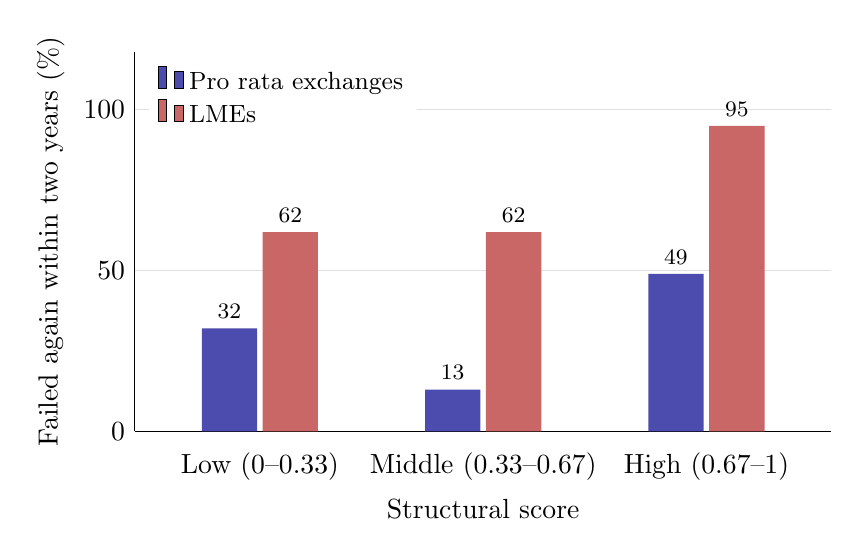
\begin{tikzpicture}
\begin{axis}[ybar, bar width=20pt, width=0.86\textwidth, height=6.4cm, ymin=0, ymax=118,
  ylabel={Failed again within two years (\%)}, symbolic x coords={Low,Middle,High}, xtick=data,
  xticklabels={{Low (0--0.33)},{Middle (0.33--0.67)},{High (0.67--1)}}, xlabel={Structural score},
  enlarge x limits=0.28, nodes near coords, nodes near coords style={font=\footnotesize},
  legend style={at={(0.02,0.98)}, anchor=north west, draw=none, font=\small}, legend cell align=left,
  ymajorgrids, grid style={gray!25}, axis lines*=left, tick style={draw=none}]
\addplot[fill=blue!55!black!70, draw=none] coordinates {(Low,32) (Middle,13) (High,49)};
\addplot[fill=red!65!black!60, draw=none] coordinates {(Low,62) (Middle,62) (High,95)};
\legend{Pro rata exchanges, LMEs}
\end{axis}
\end{tikzpicture}
\caption{Two-year failure rate by structural score and deal form}
\label{fig:bins}
\begin{minipage}{0.9\textwidth}\vspace{4pt}\footnotesize
\textit{Notes.} Deals observed for at least two years. Pro rata: $n = 44$, 15 and 82 in the low, middle and high bins; LMEs: $n = 8$, 13 and 22.
\end{minipage}
\end{figure}

Table~\ref{tab:reg_part1} reports the regression estimates. With year and industry fixed effects, moving from a score of 0 to a score of 1 raises the probability of failing within two years of a pro rata exchange by 25 percentage points (column 1; 95\% confidence interval 3 to 46 points). The three-year estimate is 20 points and the bankruptcy-only estimate 13 points, and neither is statistically significant (columns 2 and 3). In the pooled sample (column 4) the score carries a coefficient of 0.28, and doing an LME rather than a pro rata exchange raises two-year failure by a further 29 points holding the score fixed. The interaction of the score with the LME indicator is positive and insignificant ($+0.24$, $p = 0.24$).

\begin{table}[!htbp] \centering
  \caption{Structural score and post-exchange failure}
\begin{adjustbox}{max width=\textwidth}
\begin{tabular}{@{\extracolsep{5pt}}lcccc}
\\[-1.8ex]\hline
\hline \\[-1.8ex]
\\[-1.8ex] & \multicolumn{1}{c}{Fail 2y} & \multicolumn{1}{c}{Fail 3y} & \multicolumn{1}{c}{Bankrupt 2y} & \multicolumn{1}{c}{Fail 2y (pooled)}  \\
\\[-1.8ex] & (1) & (2) & (3) & (4) \\
\hline \\[-1.8ex]
 Structural score (0--1) & 0.248$^{**}$ & 0.201$^{}$ & 0.125$^{}$ & 0.275$^{***}$ \\
& (0.109) & (0.146) & (0.078) & (0.098) \\
 LME &  &  &  & 0.286$^{**}$ \\
&  &  &  & (0.115) \\
 Sample & Pro rata & Pro rata & Pro rata & All \\
 Year FE & Yes & Yes & Yes & Yes \\
 Industry FE & Yes & Yes & Yes & Yes \\
\hline \\[-1.8ex]
 Observations & 141 & 106 & 141 & 184 \\
 $R^2$ & 0.133 & 0.111 & 0.180 & 0.251 \\
\hline
\hline \\[-1.8ex]
\end{tabular}
\end{adjustbox}
\label{tab:reg_part1}
\begin{minipage}{0.95\textwidth}\vspace{4pt}\footnotesize
\textit{Notes.} Linear probability models. The structural score is the share of 70 blind re-codings that code the deal structural, counting a mixed code as one half (0 = every coder says shock, 1 = every coder says structural). Standard errors clustered by issuer in parentheses. $^{*}$p$<$0.1; $^{**}$p$<$0.05; $^{***}$p$<$0.01.
\end{minipage}
\end{table}


\paragraph{Is the relationship linear?} Not cleanly. The 15 pro rata deals in the middle third of the score fail within two years at 13\%, below both ends of the scale. In a three-bin regression with the same fixed effects, the middle bin is 10 points below the low bin ($p = 0.41$) and the high bin 19 points above it ($p = 0.05$); a quadratic term added to equation~\eqref{eq:main} is insignificant ($p = 0.41$). The data therefore cannot reject a linear relationship, but they do not confirm one, and the middle bin is too small to interpret on its own.

\paragraph{Alternative constructions.} Table~\ref{tab:robust} re-estimates column 1 of Table~\ref{tab:reg_part1} under other ways of measuring cause and on other samples. Every version gives a positive coefficient, between 0.16 and 0.37. The binary majority-wins indicator gives 0.20 ($p = 0.02$). Coder~\#1's original labels give the largest estimate (0.36), so adopting the score lowers the headline number by about a third. The estimate is weakest when the score is built from gpt-4o-mini alone (0.18, $p = 0.11$; 0.16 with the company name scrubbed) and strongest from gpt-4o alone (0.30). Restricting to each issuer's first exchange raises it to 0.35.

\begin{table}[htbp]
\centering
\caption{The structural score under alternative constructions}
\label{tab:robust}
\small
\begin{adjustbox}{max width=\textwidth}
\begin{tabular}{l r r r r}
\toprule
Specification & Coefficient & Std.\ error & $p$ & $n$ \\
\midrule
Main: continuous score & 0.248$^{**}$ & 0.109 & 0.023 & 141 \\
\addlinespace
Binary, majority wins (score $>$ 0.5) & 0.201$^{**}$ & 0.085 & 0.018 & 141 \\
High bin vs low bin (three-bin model) & 0.193$^{*}$ & 0.100 & 0.054 & 141 \\
Continuous, middle bin dropped & 0.210$^{*}$ & 0.112 & 0.061 & 126 \\
Score ignoring 'mixed' runs & 0.197$^{**}$ & 0.098 & 0.045 & 136 \\
\addlinespace
Coder \#1 on a 0 / 0.5 / 1 scale & 0.367$^{***}$ & 0.112 & 0.001 & 141 \\
Coder \#1 dummies: structural vs shock & 0.362$^{***}$ & 0.113 & 0.001 & 141 \\
\addlinespace
Score from gpt-4o-mini only & 0.183$^{}$ & 0.113 & 0.107 & 141 \\
Score from gpt-4.1-mini only & 0.240$^{**}$ & 0.097 & 0.013 & 141 \\
Score from gpt-4o only & 0.304$^{***}$ & 0.094 & 0.001 & 141 \\
Name-scrubbed score (gpt-4o-mini) & 0.157$^{}$ & 0.112 & 0.158 & 141 \\
\addlinespace
First exchange per issuer only & 0.348$^{***}$ & 0.134 & 0.009 & 108 \\
Dropping coercion-flagged pro rata deals & 0.249$^{**}$ & 0.113 & 0.028 & 134 \\
No fixed effects & 0.236$^{**}$ & 0.096 & 0.014 & 141 \\
Logit, average marginal effect (no fixed effects) & 0.237$^{**}$ & 0.095 & 0.013 & 141 \\
\bottomrule
\end{tabular}
\end{adjustbox}
\begin{minipage}{0.95\textwidth}\vspace{4pt}\footnotesize
\textit{Notes.} Dependent variable: failure within two years of a pro rata exchange. Each row is a separate linear probability model with year and industry fixed effects unless stated, standard errors clustered by issuer; the coefficient shown is on the cause measure named in the row. $^{*}$p$<$0.1; $^{**}$p$<$0.05; $^{***}$p$<$0.01.
\end{minipage}
\end{table}


\paragraph{Pre-deal credit quality.} The score is not a proxy for how weak the firm already was. Among the 142 pro rata deals with an S\&P rating one year before default, the score is essentially uncorrelated with the rating (Spearman $\rho = -0.11$, $p = 0.18$); the median rating is B$-$ in the high-score bin and CCC+ in the low-score bin. Adding the rating notch as a control gives a score coefficient of 0.31 ($p = 0.015$, $n = 124$).

\paragraph{Vintage.} Shock-coded deals cluster in 2020: the mean score of pro rata exchanges is 0.50 that year against 0.60 to 0.84 in every other year, which is why year fixed effects are included throughout. The gradient is not only a pandemic effect. It is present within the 2020 deals (50\% of high-score against 19\% of low-score deals fail; slope 0.31, $p = 0.06$) and within 2021--22 (slope 0.47, $p = 0.02$), and dropping 2020 altogether leaves a coefficient of 0.23 ($p = 0.09$, $n = 101$). It is, however, absent among the 2023 deals, the latest vintage observable at two years (39\% against 40\%; slope 0.06, $p = 0.79$, $n = 35$). Thirty-five deals cannot distinguish a weakening relationship from noise. [TODO: re-estimate when the 2024 deals reach the two-year horizon.]

\subsection{Part 2: Do lenders write different terms by cause?}
\label{sec:p2}

If lenders screen on the cause of distress, borrowers with a higher structural score should receive tougher terms than borrowers of the same vintage and industry with a lower one: more haircuts, more equity and governance to creditors, tighter documents, less sponsor-friendly runway. Table~\ref{tab:terms} reports the share of negotiated pro rata exchanges carrying each term by thirds of the score, with the LMEs alongside for comparison.

\begin{table}[htbp]\centering
\caption{Terms of the exchange by structural score}
\label{tab:terms}
\small
\begin{adjustbox}{max width=\textwidth}
\begin{tabular}{l rrr c r}
\toprule
 & \multicolumn{3}{c}{Pro rata exchanges, by structural score} & Slope $p$ & LMEs \\
 \cmidrule(lr){2-4}
Term & Low & Middle & High &  &  \\
\midrule
Haircut on exchanged claims & 45\% (49) & 38\% (13) & 47\% (83) & 0.94 & 67\% (52) \\
Debt converted to equity & 22\% (49) & 23\% (13) & 19\% (84) & 0.73 & 2\% (52) \\
Majority equity to creditors & 16\% (49) & 15\% (13) & 10\% (86) & 0.40 & 0\% (51) \\
Board / governance rights to creditors & 15\% (47) & 18\% (11) & 11\% (79) & 0.62 & 2\% (51) \\
Covenants or blockers tightened & 26\% (35) & 33\% (9) & 37\% (59) & 0.29 & 38\% (37) \\
Covenants loosened or waived & 37\% (35) & 67\% (9) & 56\% (59) & 0.09 & 65\% (37) \\
Priming new money & 19\% (47) & 23\% (13) & 37\% (79) & 0.09 & 88\% (52) \\
Any new money & 43\% (49) & 77\% (13) & 59\% (85) & 0.13 & 94\% (52) \\
Maturity extended & 73\% (44) & 50\% (12) & 69\% (70) & 0.51 & 68\% (44) \\
PIK / payment-in-kind coupon & 50\% (42) & 64\% (11) & 64\% (67) & 0.16 & 62\% (39) \\
Coupon increased & 31\% (42) & 36\% (11) & 28\% (67) & 0.92 & 31\% (39) \\
Sponsor contribution & 18\% (38) & 55\% (11) & 31\% (67) & 0.18 & 25\% (40) \\
Unequal treatment of holders & 38\% (48) & 23\% (13) & 47\% (83) & 0.36 & 90\% (51) \\
\midrule
Control index (0--5) & 1.08 (49) & 1.00 (13) & 1.10 (86) & 0.99 & 1.67 (52) \\
Ownership index (0--3) & 0.49 (49) & 0.54 (13) & 0.47 (86) & 0.92 & 0.29 (52) \\
Runway index (0--4) & 1.52 (48) & 1.92 (13) & 1.73 (84) & 0.36 & 1.69 (52) \\
Strictness index (s.d.\ units) & 0.04 (49) & -0.06 (13) & 0.04 (86) & 0.97 & -- \\
\bottomrule
\end{tabular}
\end{adjustbox}
\begin{minipage}{0.95\textwidth}\vspace{4pt}\footnotesize
\textit{Notes.} Negotiated deals only (open-market repurchases excluded): 148 pro rata exchanges with a structural score (49 low, 0--0.33; 13 middle; 86 high, 0.67--1) and 52 LMEs. Each cell is the share of deals with the term among deals whose release states it; the number stated is in parentheses. Slope $p$ is the $p$-value on the structural score in a bivariate regression of the term on the score, issuer-clustered. The strictness index is the Kling--Liebman--Katz standardised index; higher is tougher on the borrower.
\end{minipage}
\end{table}


There is no visible gradient in the control terms. High-score firms are no more likely than low-score firms to take a haircut (47\% against 45\%), to hand majority equity to creditors (10\% against 16\%) or to grant governance rights (11\% against 15\%); their documents are tightened somewhat more often (37\% against 26\%). None of the thirteen bivariate slopes on the score is significant at the 5\% level, and of the two with $p < 0.10$ one runs in the borrower-friendly direction (covenants loosened or waived, 56\% against 37\%) and the other is priming new money (37\% against 19\%). The control index averages 1.08 for low-score and 1.10 for high-score firms (slope $p = 0.99$), and the standardised strictness index, which uses every deal and corrects for how many terms a release happens to mention, is 0.04 in both.

What \emph{does} move the terms is the form of the deal. The LME column of Table~\ref{tab:terms} looks nothing like the pro rata columns: 88\% of LMEs involve priming new money, 90\% treat holders unequally, 67\% impose a haircut on non-participants, and none---0 of 51---transfers majority equity to creditors. Deal form, not diagnosis, determines what lenders extract.

Table~\ref{tab:reg_terms} adds year and industry fixed effects. The coefficient on the structural score is small and insignificant for a haircut ($+0.03$, $p = 0.76$), control equity ($-0.03$, $p = 0.71$) and priming new money ($+0.04$, $p = 0.67$), as it is for the control index ($+0.12$ on a scale whose mean is about one, $p = 0.60$) and the strictness index ($+0.09$ standard deviations, $p = 0.46$). The one term that moves is documents tightened ($+0.25$, $p = 0.06$), estimated on the 103 deals whose release describes the covenants. That is the only sign of screening on cause in the data, and it is marginal.

\begin{table}[!htbp] \centering
  \caption{Do lenders write different terms by cause of distress?}
\begin{adjustbox}{max width=\textwidth}
\begin{tabular}{@{\extracolsep{2pt}}lcccccc}
\\[-1.8ex]\hline
\hline \\[-1.8ex]
\\[-1.8ex] & \multicolumn{1}{c}{Haircut} & \multicolumn{1}{c}{Control equity} & \multicolumn{1}{c}{Docs tightened} & \multicolumn{1}{c}{Priming new money} & \multicolumn{1}{c}{Control index} & \multicolumn{1}{c}{Strictness index}  \\
\\[-1.8ex] & (1) & (2) & (3) & (4) & (5) & (6) \\
\hline \\[-1.8ex]
 Structural score (0--1) & 0.034$^{}$ & -0.028$^{}$ & 0.250$^{*}$ & 0.042$^{}$ & 0.123$^{}$ & 0.091$^{}$ \\
& (0.111) & (0.076) & (0.133) & (0.100) & (0.236) & (0.123) \\
 Year FE & Yes & Yes & Yes & Yes & Yes & Yes \\
 Industry FE & Yes & Yes & Yes & Yes & Yes & Yes \\
\hline \\[-1.8ex]
 Observations & 145 & 148 & 103 & 139 & 148 & 148 \\
 $R^2$ & 0.165 & 0.258 & 0.175 & 0.269 & 0.188 & 0.203 \\
\hline
\hline \\[-1.8ex]
\end{tabular}
\end{adjustbox}
\label{tab:reg_terms}
\begin{minipage}{0.95\textwidth}\vspace{4pt}\footnotesize
\textit{Notes.} Negotiated pro rata exchanges with a structural score. Cols.\ 1--4 LPMs, cols.\ 5--6 OLS on the index. Standard errors clustered by issuer in parentheses. $^{*}$p$<$0.1; $^{**}$p$<$0.05; $^{***}$p$<$0.01.
\end{minipage}
\end{table}


Two qualifications apply to reading these as a null. First, the test is not powerful: with 148 deals, and fewer where the documents are described, the smallest score effect detectable at 80\% power is roughly 30--35 percentage points on any one term, so the evidence rules out large cause-based screening but not modest screening. The 95\% confidence interval on the control-index coefficient runs from $-0.34$ to $+0.59$ on a scale whose mean is about one. Second, the terms are coded from rating-agency releases, which describe covenant changes inconsistently; that measurement error biases every coefficient toward zero, and a document-layer coding from the credit agreements themselves is the natural next step. The correct statement is therefore that lenders' terms do not \emph{detectably} vary with cause, not that they do not vary at all.

\paragraph{Vintage.} Table~\ref{tab:vintage} shows that pro rata terms have drifted toward LME-style structures over time. Between 2018--21 and 2023--25 the share of deals giving creditors any equity fell from 49\% to 25\% ($p = 0.005$), while PIK coupons rose from 48\% to 75\% ($p = 0.004$) and priming new money from 12\% to 48\% ($p < 0.001$). Documents-tightened was flat at about a third. The cause mix also shifted toward structural firms in the later period (mean structural score 0.68 against 0.55), which is why year fixed effects are included throughout; the vintage shift is not, however, a cause shift in disguise, since within-year the cause gradient in terms remains absent.

\begin{table}[htbp]\centering
\caption{Pro rata exchange terms by vintage}
\label{tab:vintage}
\small
\begin{tabular}{l rr r r}
\toprule
Term & 2018--21 & 2023--25 & Change (pp) & Fisher $p$ \\
\midrule
Any equity to creditors & 49\% (73) & 25\% (67) & -24 & 0.01 \\
Debt converted to equity & 26\% (72) & 12\% (66) & -14 & 0.05 \\
Haircut on exchanged claims & 51\% (72) & 40\% (65) & -11 & 0.23 \\
PIK / payment-in-kind coupon & 48\% (61) & 75\% (53) & +28 & 0.00 \\
Maturity extended & 61\% (59) & 74\% (61) & +13 & 0.17 \\
Priming new money & 12\% (68) & 48\% (64) & +37 & 0.00 \\
Covenants or blockers tightened & 31\% (51) & 35\% (46) & +3 & 0.83 \\
Covenants loosened or waived & 47\% (51) & 57\% (46) & +9 & 0.42 \\
Sponsor contribution & 25\% (57) & 36\% (53) & +11 & 0.22 \\
\midrule
Share of deals coded A / B / C & 37\% / 42\% / 21\% & 21\% / 54\% / 25\% & & \\
\bottomrule
\end{tabular}
\begin{minipage}{0.9\textwidth}\vspace{4pt}\footnotesize
\textit{Notes.} Negotiated pro rata exchanges; 2022 deals (8) omitted from the two columns. Shares among deals whose release states the term; number stated in parentheses.
\end{minipage}
\end{table}

\paragraph{Is whatever screening exists enough?} The sharpest test of whether lenders are already pricing cause into the deal is to ask whether the terms absorb the cause effect on outcomes. If tough terms were being allocated to the firms whose diagnosis predicts failure, then conditional on the terms the cause of distress should no longer predict failure. Table~\ref{tab:absorb} runs this test. Deals that actually reduce debt---a haircut or equitisation---fail within two years at 29\% against 51\% for deals that only buy time with an extension or PIK coupon, and the balance-sheet-fix indicator carries a coefficient of $-0.24$ ($p < 0.01$) with year fixed effects. One standard deviation of the strictness index lowers two-year failure by 28 percentage points ($p < 0.001$). Yet adding either measure leaves the coefficient on the structural score essentially unchanged: $+0.22$ with the strictness index and $+0.21$ with the balance-sheet-fix indicator, against $+0.22$ without the terms. The terms matter a great deal for whether the exchange holds; they are simply not being directed at the firms whose cause of distress says they will not.

\begin{table}[!htbp] \centering
  \caption{Do the terms absorb the cause effect? Two-year failure on terms and the structural score}
\begin{adjustbox}{max width=\textwidth}
\begin{tabular}{@{\extracolsep{5pt}}lcccc}
\\[-1.8ex]\hline
\hline \\[-1.8ex]
\\[-1.8ex] & \multicolumn{1}{c}{Fail 2y} & \multicolumn{1}{c}{Fail 2y} & \multicolumn{1}{c}{Fail 2y} & \multicolumn{1}{c}{Fail 2y}  \\
\\[-1.8ex] & (1) & (2) & (3) & (4) \\
\hline \\[-1.8ex]
 Balance-sheet fix & -0.243$^{***}$ & -0.243$^{***}$ &  &  \\
& (0.092) & (0.092) &  &  \\
 Strictness index &  &  &  & -0.277$^{***}$ \\
&  &  &  & (0.066) \\
 Structural score (0--1) &  & 0.210$^{*}$ & 0.224$^{**}$ & 0.222$^{**}$ \\
&  & (0.110) & (0.105) & (0.099) \\
 Year FE & Yes & Yes & Yes & Yes \\
\hline \\[-1.8ex]
 Observations & 102 & 102 & 107 & 107 \\
 $R^2$ & 0.145 & 0.175 & 0.107 & 0.199 \\
\hline
\hline \\[-1.8ex]
\end{tabular}
\end{adjustbox}
\label{tab:absorb}
\begin{minipage}{0.95\textwidth}\vspace{4pt}\footnotesize
\textit{Notes.} Negotiated pro rata exchanges eligible at two years; cols.\ 1--2 drop deals with relief type not stated. LPMs; SEs clustered by issuer. Balance-sheet fix = haircut or equitisation; strictness in s.d.\ units. $^{*}$p$<$0.1; $^{**}$p$<$0.05; $^{***}$p$<$0.01.
\end{minipage}
\end{table}


The combination of a positive, stable cause effect on outcomes (Section~\ref{sec:p1}) with no detectable cause effect on terms is the central result of Part~2. One reading consistent with \citet{kahl2002} should be kept in view: a lender who cannot yet tell which kind of distress it faces may rationally grant a short extension and pull the plug later, so that a structural firm's subsequent failure is the plan working rather than the screen failing. That account cannot be distinguished from a failure to screen without data on recoveries, which this paper does not observe.

% ---------------------------------------------------------------------
\section{Discussion}
% ---------------------------------------------------------------------
[TODO: interpretation; what the results say about lenders' consent; limitations (sample size and power in Part 2; terms coded from rating-agency releases, which under-report covenant changes and bias Part 2 toward zero; confidential issuers; document-layer terms not yet coded); future work.]

% ---------------------------------------------------------------------
\section{Conclusion}
% ---------------------------------------------------------------------
[TODO]

\bibliography{references}

\appendix
\section{Cause-of-distress codebook}
\label{app:codebook}

\noindent\textbf{Unit.} One distressed exchange. Evidence: S\&P and Moody's rating-action rationales in the 12 months before the deal; the agencies' statement of the EBITDA trend over the prior two years; secondary factors named.

\medskip\noindent\textbf{A --- Shock} (temporary; the business model is intact, the problem is expected to pass or is purely financial).
\begin{description}
  \item[A1 Demand / operating shock.] An identifiable external event hit demand, prices or operations (pandemic, commodity-price collapse, hurricane, strike, a one-off customer loss) and the agency language treats it as cyclical or temporary.
  \item[A2 Financial shock.] The operating business is stable (EBITDA flat or up) but the capital structure is the problem: buyout leverage, a maturity wall, refinancing risk, floating-rate interest burden, a covenant breach with stable EBITDA.
\end{description}

\noindent\textbf{B --- Structural} (the business itself is impaired and the agency does not expect it to recover on its own).
\begin{description}
  \item[B1 Secular industry decline.] The whole industry is shrinking (print media, department stores, coal, landline telecom, offshore drilling after 2014).
  \item[B2 Firm-specific deterioration.] Competitive losses, failed strategy, botched integration, lost contracts, management failures: the firm is declining while its industry is not.
  \item[B3 Legal / regulatory.] Litigation, regulatory change or government action is the primary driver (opioid liability, reimbursement cuts, loss of a licence).
\end{description}

\noindent\textbf{C --- Mixed.} An A-type shock landed on a firm that already had B-type problems, and neither clearly dominates.

\medskip\noindent\textbf{Tie-break rules, applied in order.}
\begin{enumerate}
  \item Identify the \emph{primary} driver the agency names. If one driver is clearly primary, code it; secondary factors do not change the letter.
  \item \emph{EBITDA rule.} If EBITDA fell by more than about 10\% over the two years before the deal \emph{and} the agency attributes the fall to the business rather than to an external event, lean B. If EBITDA is flat or up, lean A2.
  \item \emph{COVID rule.} A 2020--21 deal in which the agency names the pandemic as primary is A1 unless the issuer was already on negative outlook or downgraded for operating reasons in the 24 months before March 2020, in which case it is C.
  \item \emph{LBO rule.} Leverage from a buyout or dividend recapitalisation on a stable business is A2, not B2.
  \item If an external shock and a pre-existing structural problem are given roughly equal weight, code C.
\end{enumerate}

\noindent\textbf{Recorded for every deal.} Code; confidence (High / Medium / Low); primary driver; secondary drivers; verbatim agency language relied on, with agency and month; EBITDA trend; sources.

\noindent\textbf{Repeat exchanges} by the same issuer are coded separately for each deal's own twelve-month window.

\medskip\noindent\textbf{From codes to the structural score.} Each deal is coded 70 times with this codebook (30 runs each of two models and 10 of a third, blind to the deal's form and outcome). The structural score is the number of runs coded B plus half the number coded C, divided by 70: 0 if every run codes A, 1 if every run codes B. The score, not any single letter, is the cause measure used in the main specifications (Section~\ref{sec:score}).

\end{document}
